%!TEX root=../main.tex	% Optional

\section{JavaEE}
\subsection{General}

Die \textbf{Java Platform Enterprise Edition} enthält Spezifikationen welche die Java SE (\textbf{Java Standard Edition}) erweitert.

Diese Spezifikationen sind beispielsweise Funktionen wie \textit{Distributed Computing} und \textit{Web Services}.

Eine Java EE Application wird auf Application Server oder Microservices ausgeführt.

Siehe: \cite{wiki:javaee}


Die einzelnen Java EE Spezifikationen sind ebenfalls unterteilt in folgende Unterpunkte:

\begin{itemize}
    \item Web Specifications
        \subitem Servlet: HTTP Request Manager
        \subitem Java Server Faces: Generierte UI aus Komponenten
        \subitem Unified Expression Language: Web Sprache um Komponenten zu verbinden
    \item Web service Specifications
        \subitem REST Schnittstellen
        \subitem JSON Schnittstellen
        \subitem XML Schnittstellen
    \item Enterprise Specifications
        \subitem Dependency Injection tools
        \subitem Enterprise Java Bean
    \item Other Specifications
        \subitem Validation: Validierung verschiedener Properties wie z.B.: eMail
\end{itemize}


\subsection{Formate}

Außerdem werden Java EE Applications in verschiedene Paket Formate verpackt:

\begin{itemize}
    \item .WAR: \textbf{W}eb \textbf{A}pplication \textbf{R}esources oder \textbf{W}eb \textbf{Ar}chives - Benutzt für web Applikationen wie zum Beispiel eine Glassfish Applikation
    \item .RAR: \textbf{R}esource \textbf{A}dapte\textbf{r}s
    \item .EAR: \textbf{E}nterprise \textbf{A}pplication \textbf{R}esources
    \item lib/: normale JAR files
\end{itemize}

JavaEE ist von der Struktur her folgendermaßen aufgebaut:

\begin{figure}
    \centering
    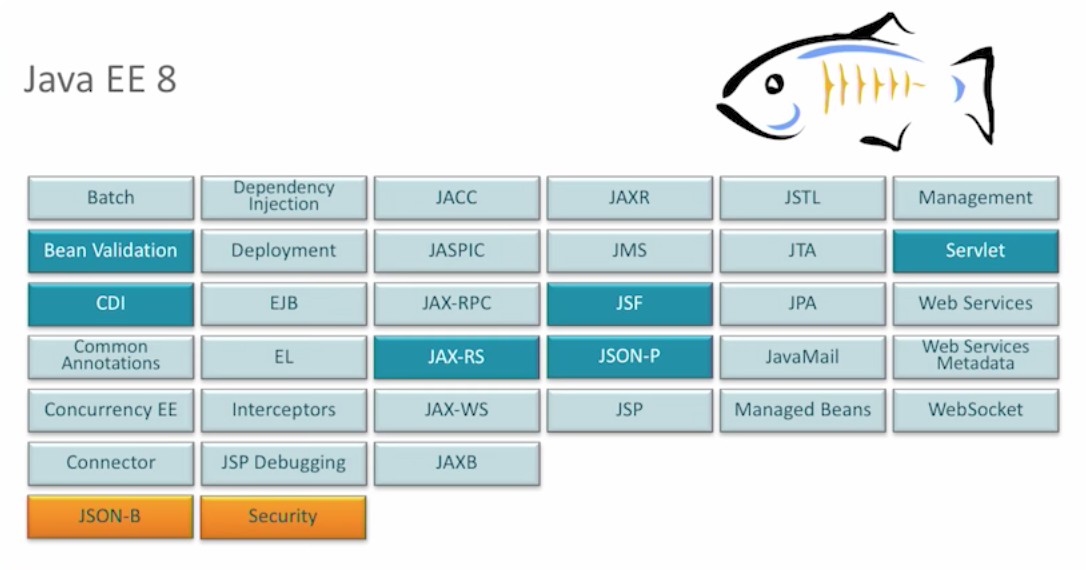
\includegraphics[width=\textwidth]{images/javaee-overview1}
    \caption{JavaEE 8 Overview von Oracle Blogs \cite{stackoverflow:javaee}}
\end{figure}

\begin{figure}
    \centering
    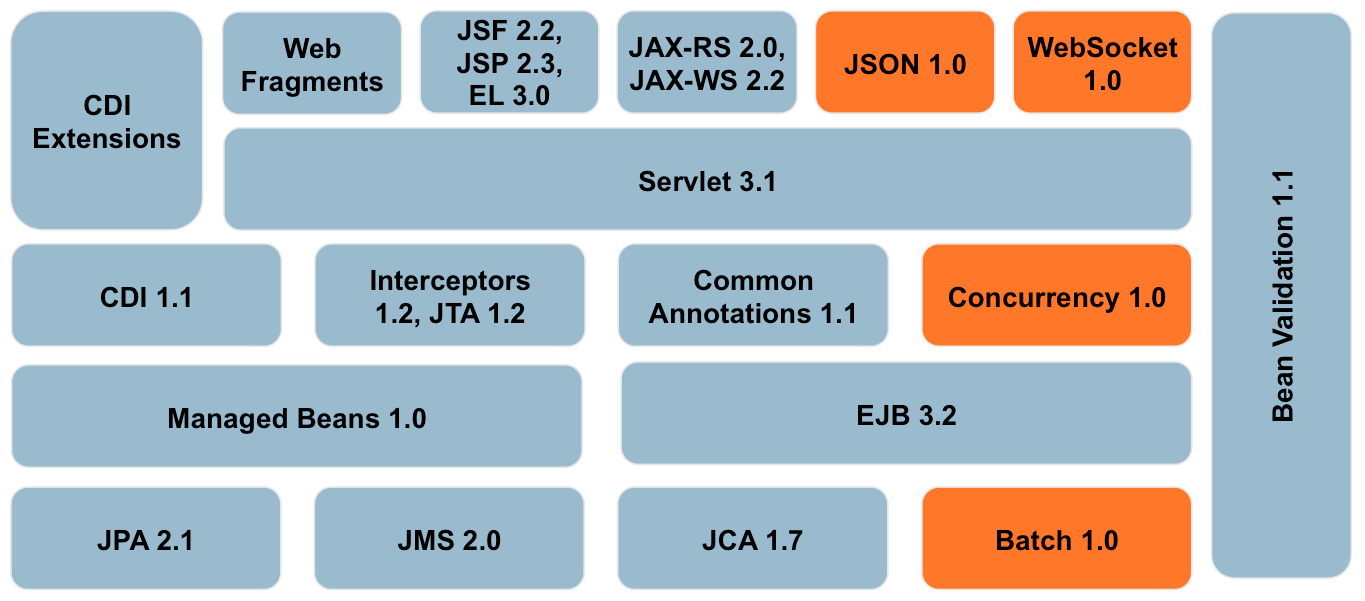
\includegraphics[width=\textwidth]{images/javaee-overview2}
    \caption{JavaEE 8 Overview von Java Road Tripping \cite{stackoverflow:javaee}}
\end{figure}

\clearpage
\section{Application Server}

\subsection{Glassfish}

Als Runtime für die \textbf{JavaEE Web Application} verwenden wir den \textit{Application Server} \textbf{Glassfish} \cite{github:glassfish}.

\textbf{Glassfish} ist eine referenz implementierung von \textbf{Java EE} und unterstützt deshalb \textit{Enterprise JavaBeans}, \textit{JPA}, \textit{JavaServer Faces}, \textit{JMS}, \textit{RMI}, \textit{JavaServer Pages}, \textit{servlets}, und mehr \textbf{Java EE} Spezifikationen.

Das Backend von \textbf{Glassfish} läuft auf einem Apache Tomcat Server.

Die neueste Glassfish Version ist 5.0, welche im September 2017 erschienen ist.

\subsection{Glassfish Setup}

Der \textbf{Glassfish} Application Server soll in einem Docker Container gestartet werden, hierzu verwende ich das Dockerfile von Oracle \cite{github:oracle-docker-images}.

\begin{code}{sh}
    git clone https://github.com/oracle/docker-images/
    cd docker-images/GlassFish/5.0
    docker build -t glassfish5 .  # Container Builden
    docker run -d -p 4848:4848 -p 8080:8080 -p 8181:8181 -p 9009:9009 glassfish5  # Container starten
    xdg-open http://127.0.0.1:4848/  # Website starten
\end{code}

Der standard Benutzername ist \texttt{admin}, das Passwort ist \texttt{admin}.

Die Glassfish Startseite sieht folgendermaßen aus:

\begin{figure}
    \centering
    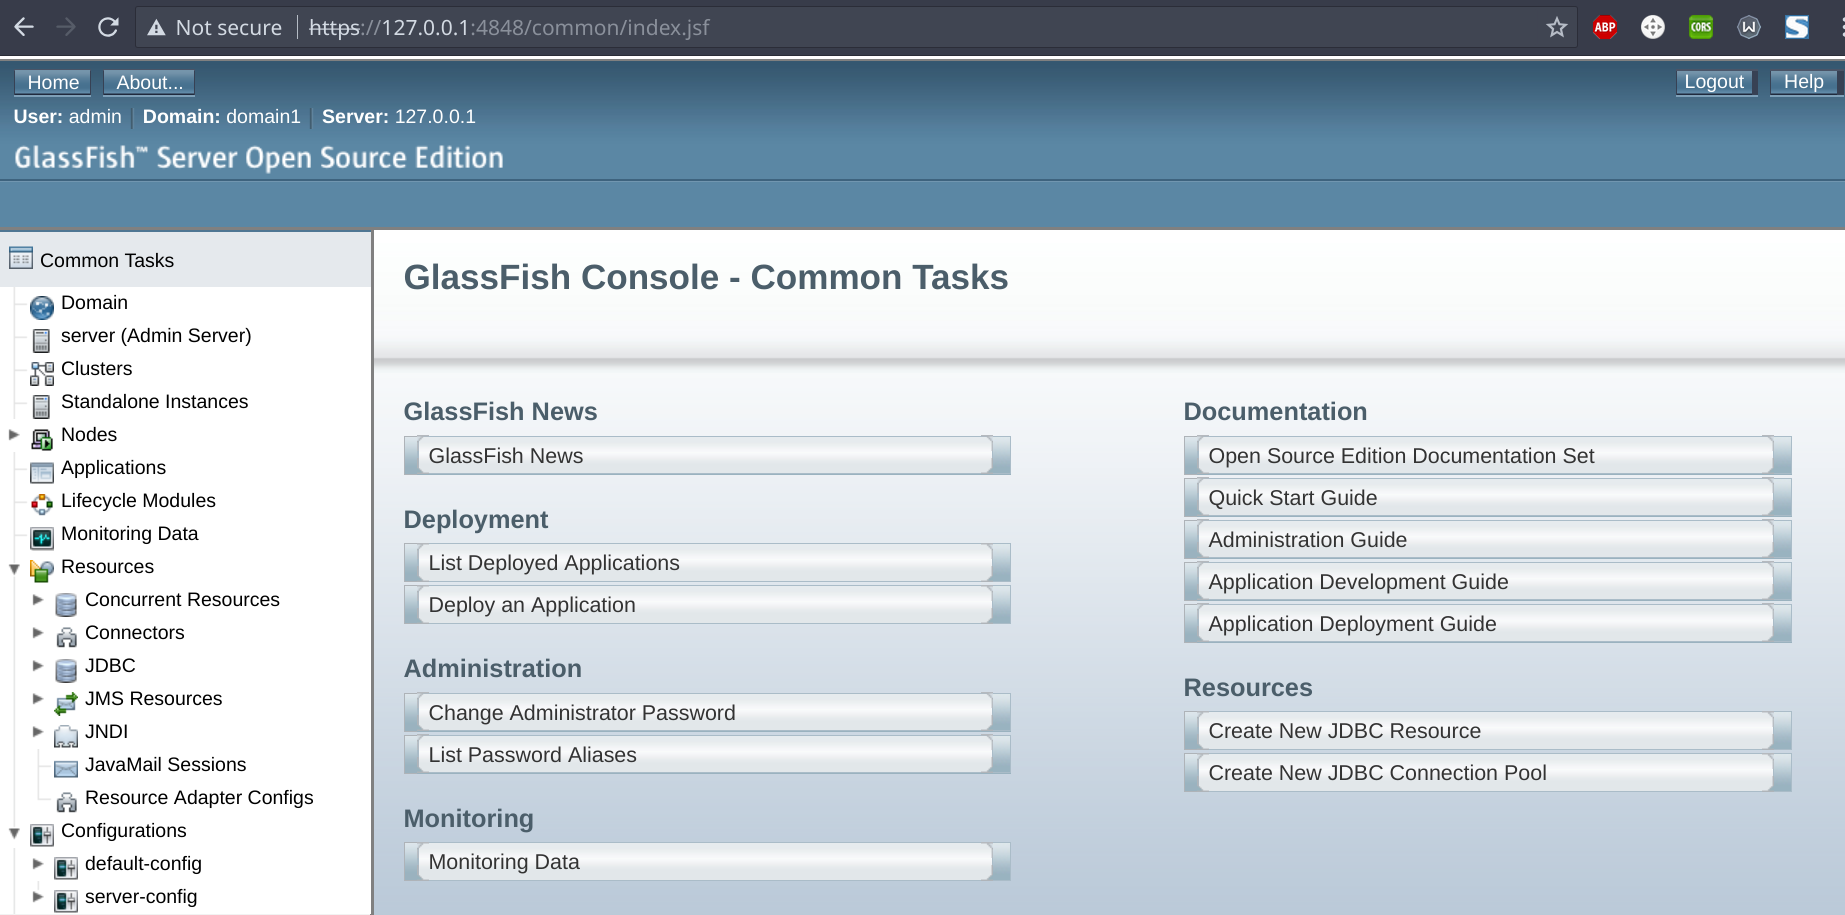
\includegraphics[width=\textwidth]{images/glassfish-home}
    \caption{Glassfish Startseite}
\end{figure}




\clearpage
\section{Deploy}

\subsection{JavaEE Examples Repository}

Nun können wir eine JavaEE Applikation auf den Application Server deployen. Diese läuft dann unter der Glassfish JavaEE runtime welche zusätzliche Sicherheitsmaßnahmen und sonstige benötigte Features vorweist.

\begin{code}{sh}
    git clone https://github.com/javaee/tutorial-examples
    cd tutorial-examples
    mvn package
    cd web/jsf/ajaxguessnumber
\end{code}

Wir werden die Web Application \textbf{Ajax Guess Number} deployen.

\subsection{Java Annotations}

Ein Controller ist eine normale Java Klasse (POJO), welche mit Annotations zu einem Controller aufgerüstet werden kann.

Hierbei gibt es Beispielsweise die Annotation \texttt{@Named}:

\begin{code}{java}
    @Named
    public class UserNumberBean implements Serializable {
        ...
    }
\end{code}

Außerdem sollten wir den Scope spezifizieren, wobei man unterscheidet zwischen \texttt{@RequestScoped}, welches eine neue Instanz pro Anfrage ("Request") erstellt, und \texttt{@SessionScoped}, welche eine Sitzung erstellt um mögliche Properties oder Variablen beizubehalten.

\begin{code}{java}
    @Named
    @RequestScoped
    public class UserNumberBean implements Serializable {
        ...
    }
\end{code}

Außerdem können wir dem \texttt{UserNumberBean} Controller eine Instanz eines Objektes zuteilen, welche von \textbf{JavaEE} automatisch injiziert wird:


\texttt{UserNumberBean.java}
\begin{code}{java}
    @Named
    @RequestScoped
    public class UserNumberBean implements Serializable {
        // JavaEE kümmert sich um das erstellen der Instanz
        @Inject
        DukesNumberBean dukesNumberBean;
    }
\end{code}

\texttt{DukesNumberBean.java}
\begin{code}{java}
    @Named
    @SessionScoped
    public class DukesNumberBean implements Serializable {

        private static final long serialVersionUID = 6575056551121951958L;
        private Integer randomInt = null;
        private long maximum = 10;
        private long minimum = 0;

        public DukesNumberBean() {
            Random randomGR = new Random();
            long range = maximum + minimum + 1;
            randomInt = (int) (minimum + randomGR.nextDouble() * range);
            System.out.println("Duke's number: " + randomInt);
        }

        ...
    }
\end{code}

\subsection{Response}

In dem \texttt{UserNumberBean} Controller müssen wir bloß noch eine Response, also eine Plain-Text HTTP Antwort, zurückgeben, welches mit der \texttt{getResponse} methode geschieht:

\begin{code}{java}
    @Named
    @RequestScoped
    public class UserNumberBean implements Serializable {
        @Inject
        DukesNumberBean dukesNumberBean;
        private Integer userNumber = null;
        String response = null;

        public String getResponse() {
            int random = dukesNumberBean.getRandomInt();
            if ((userNumber != null)
                    && (userNumber.compareTo(random) == 0)) {
                return "Yay! You got it!";
            }
            if (userNumber == null) {
                return null;
            } else {
                return "The random number is " +
                        (random > userNumber ? "greater" : "smaller") +
                        " than your guess";
            }
        }

        ...
    }
\end{code}

\subsection{WAR Build}
Nun muss eine \texttt{.war} Datei erstellt werden, welche dann auf dem \textbf{Glassfish} server läuft.

\begin{figure}
    \centering
    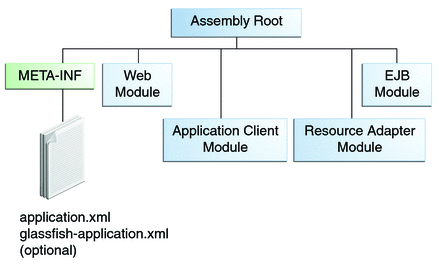
\includegraphics[width=\textwidth]{images/war-overview}
    \caption{JavaEE WAR Overview \cite{javaee:war}}
\end{figure}


Hierzu verwenden wir das Maven WAR Plugin in der \texttt{pom.xml} file:

\begin{code}{xml}
    <plugin>
        <artifactId>maven-war-plugin</artifactId>
        <configuration>
            <attachClasses>true</attachClasses>
            <webXml>target/web.xml</webXml>
            <webResources>
                <resource>
                    <directory>src/main/webapp</directory>
                    <filtering>true</filtering>
                </resource>
            </webResources>
        </configuration>
    </plugin>
\end{code}

Beim kompilieren wird nun auch ein \texttt{.war} (Web Archive/Web Application Resource) file erstellt, welche nun auf den Glassfish Server deployed wird.

\subsection{WAR Deploy}

Der Menüpunkt \textit{Deploy an Application} leitet auf folgende Seite weiter:

\begin{figure}
    \centering
    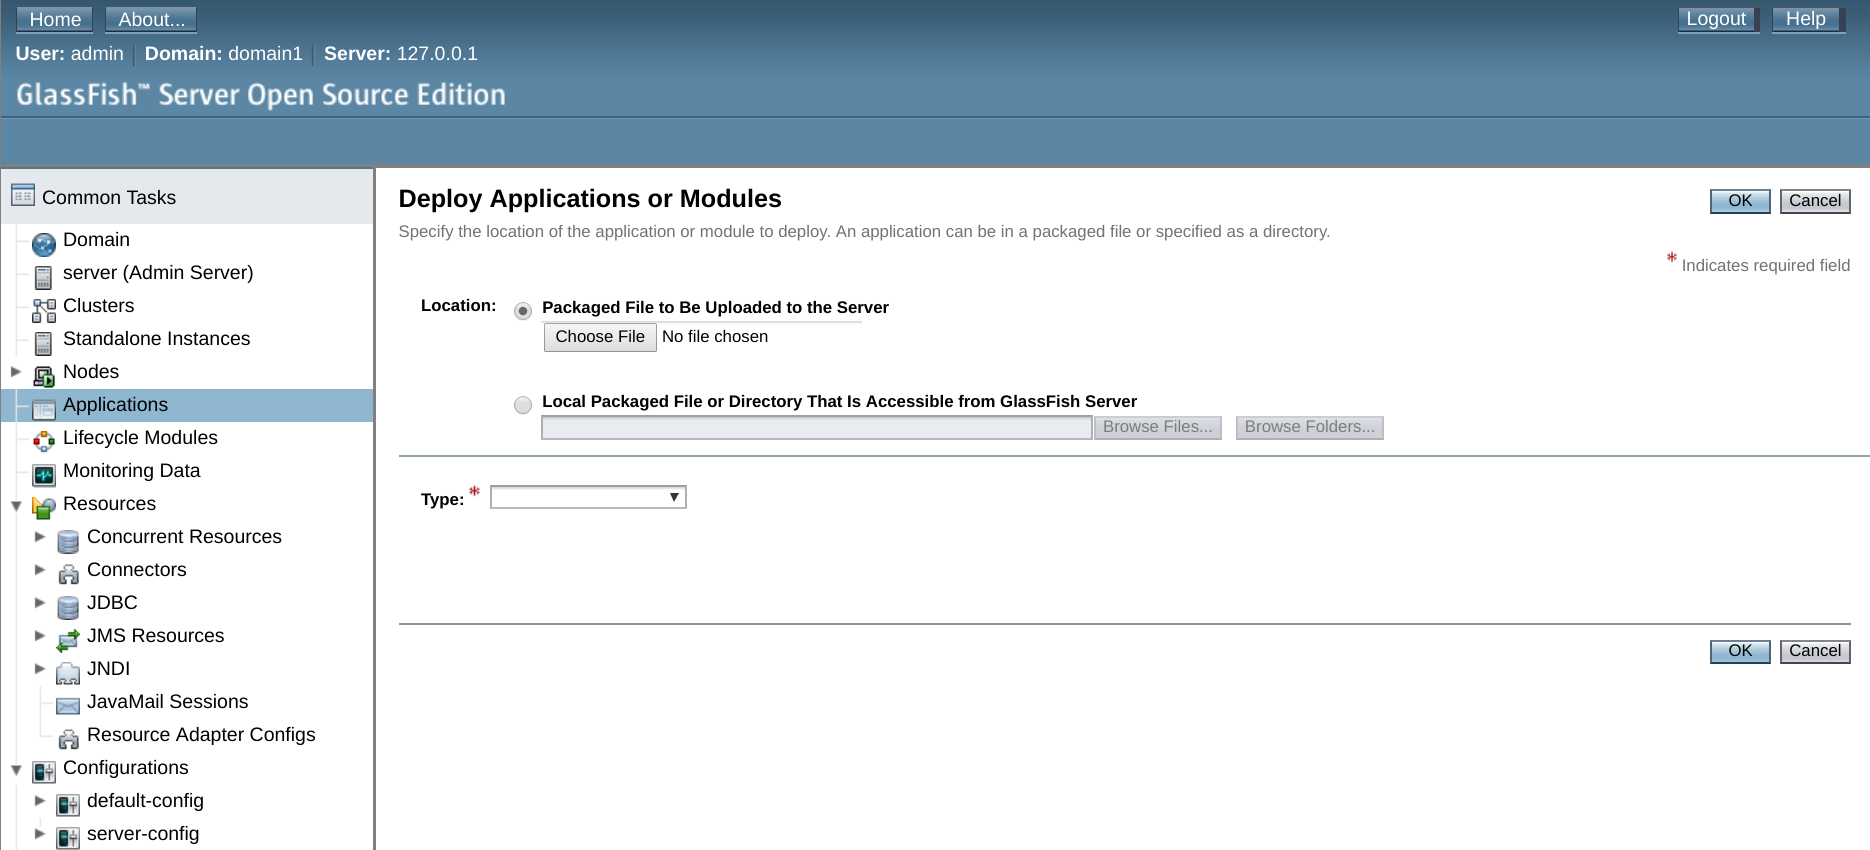
\includegraphics[width=\textwidth]{images/glassfish-deploy}
    \caption{Glassfish - Deploy an Application}
\end{figure}

Das \texttt{war} Package muss ausgewählt und hochgeladen werden, und der Typ muss auf \textit{Web Application} gesetzt sein. Nun wird die Application im \textbf{Glassfish Application Pool} laufen.

\begin{figure}
    \centering
    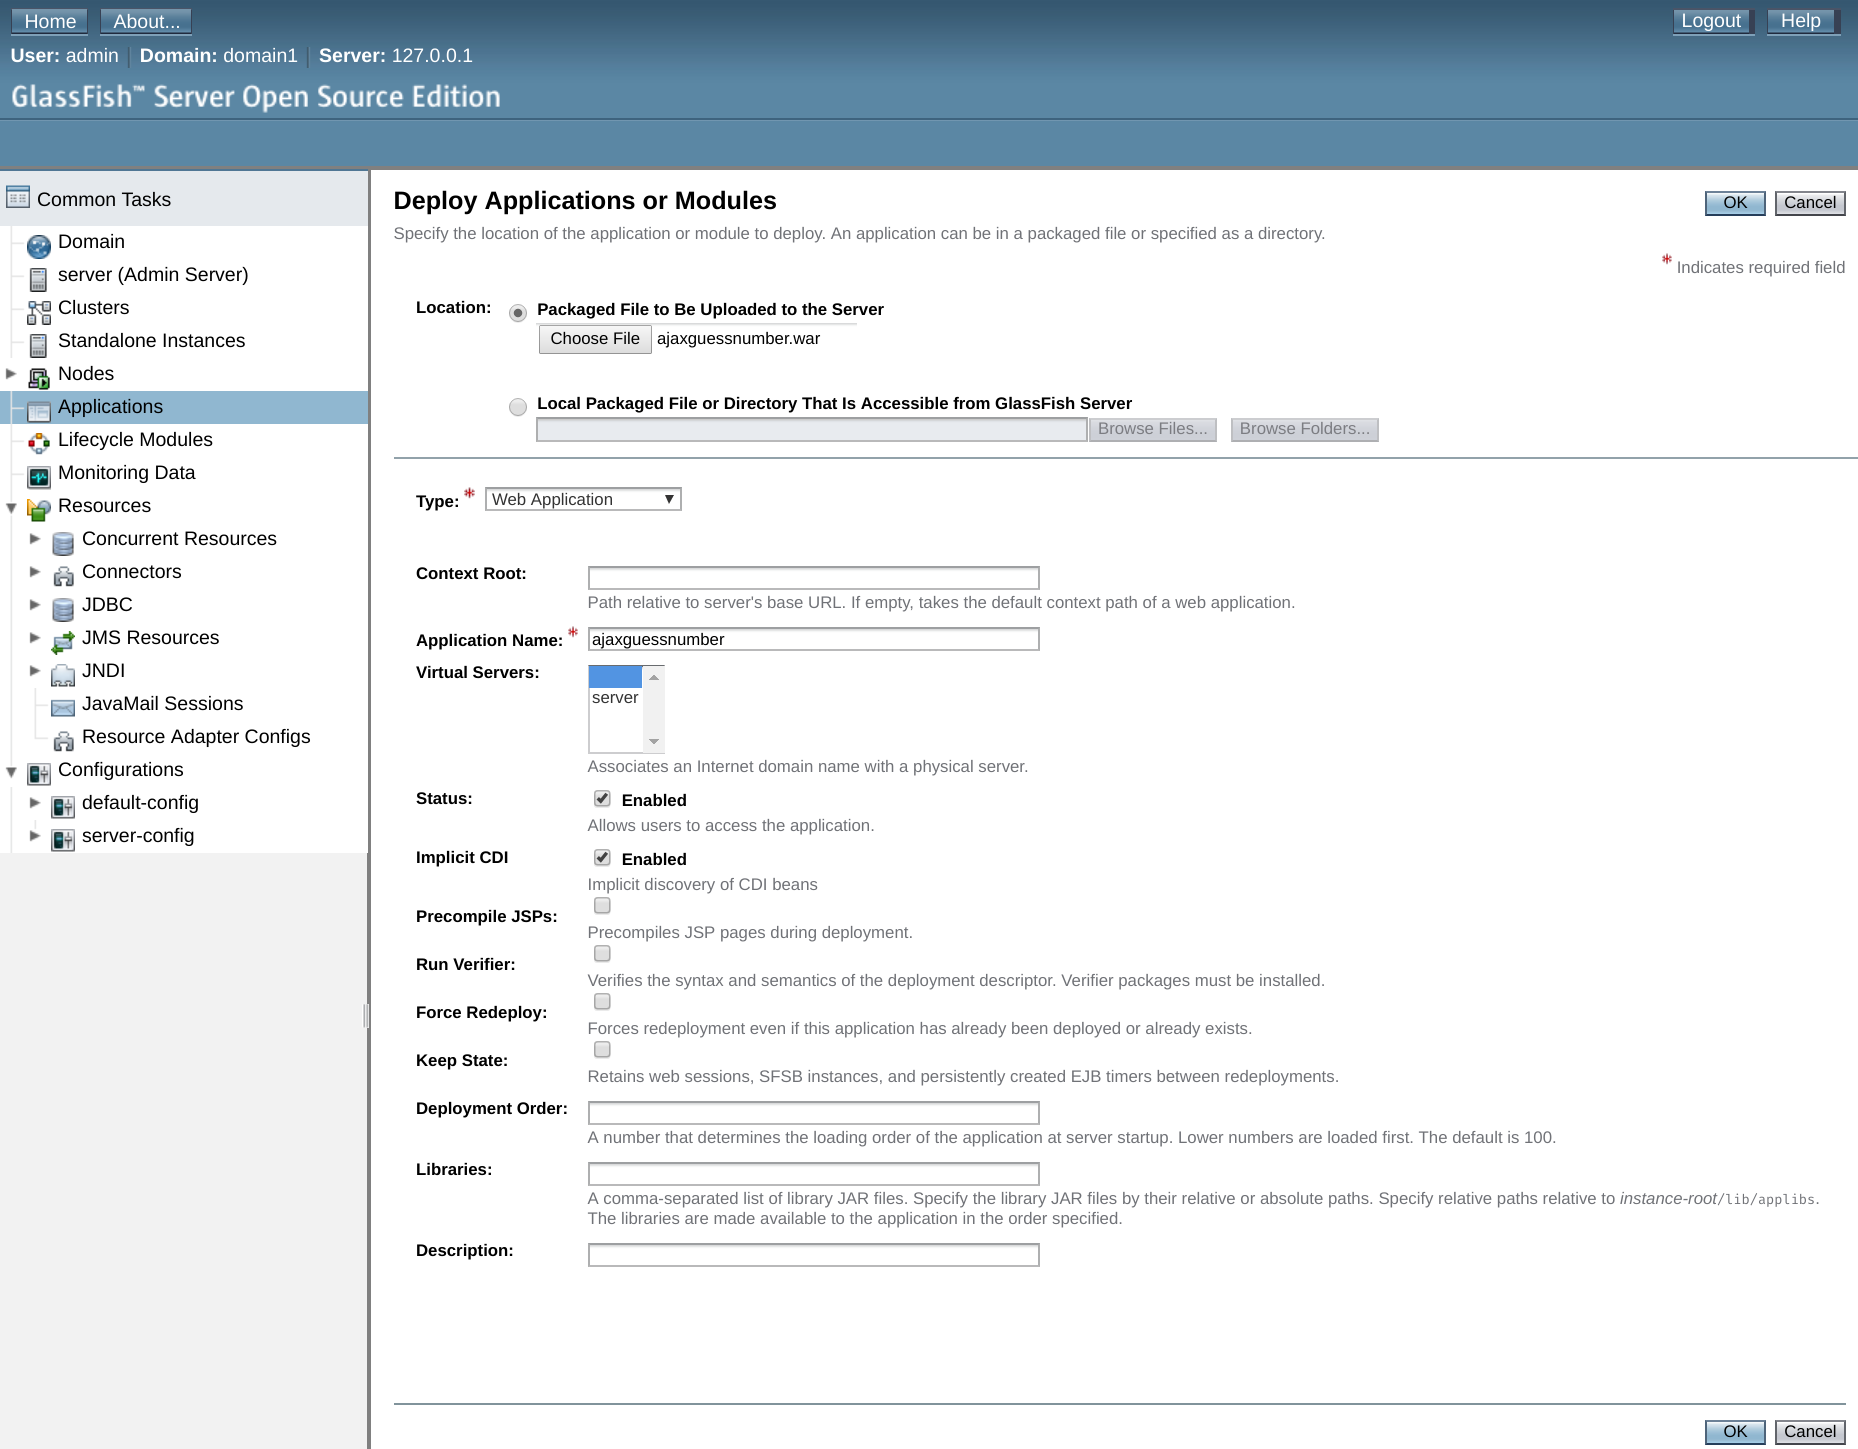
\includegraphics[width=\textwidth]{images/glassfish-deploy-war}
    \caption{Glassfish - Deploy an Application - Settings}
\end{figure}

\subsection{Glassfish Management}

Alle Applications sind einsehbar unter dem Menüpunkt \textit{List Deployed Applications}, wo sie auch gestartet, erneut deployed und erneut geladen werden können.

\begin{figure}
    \centering
    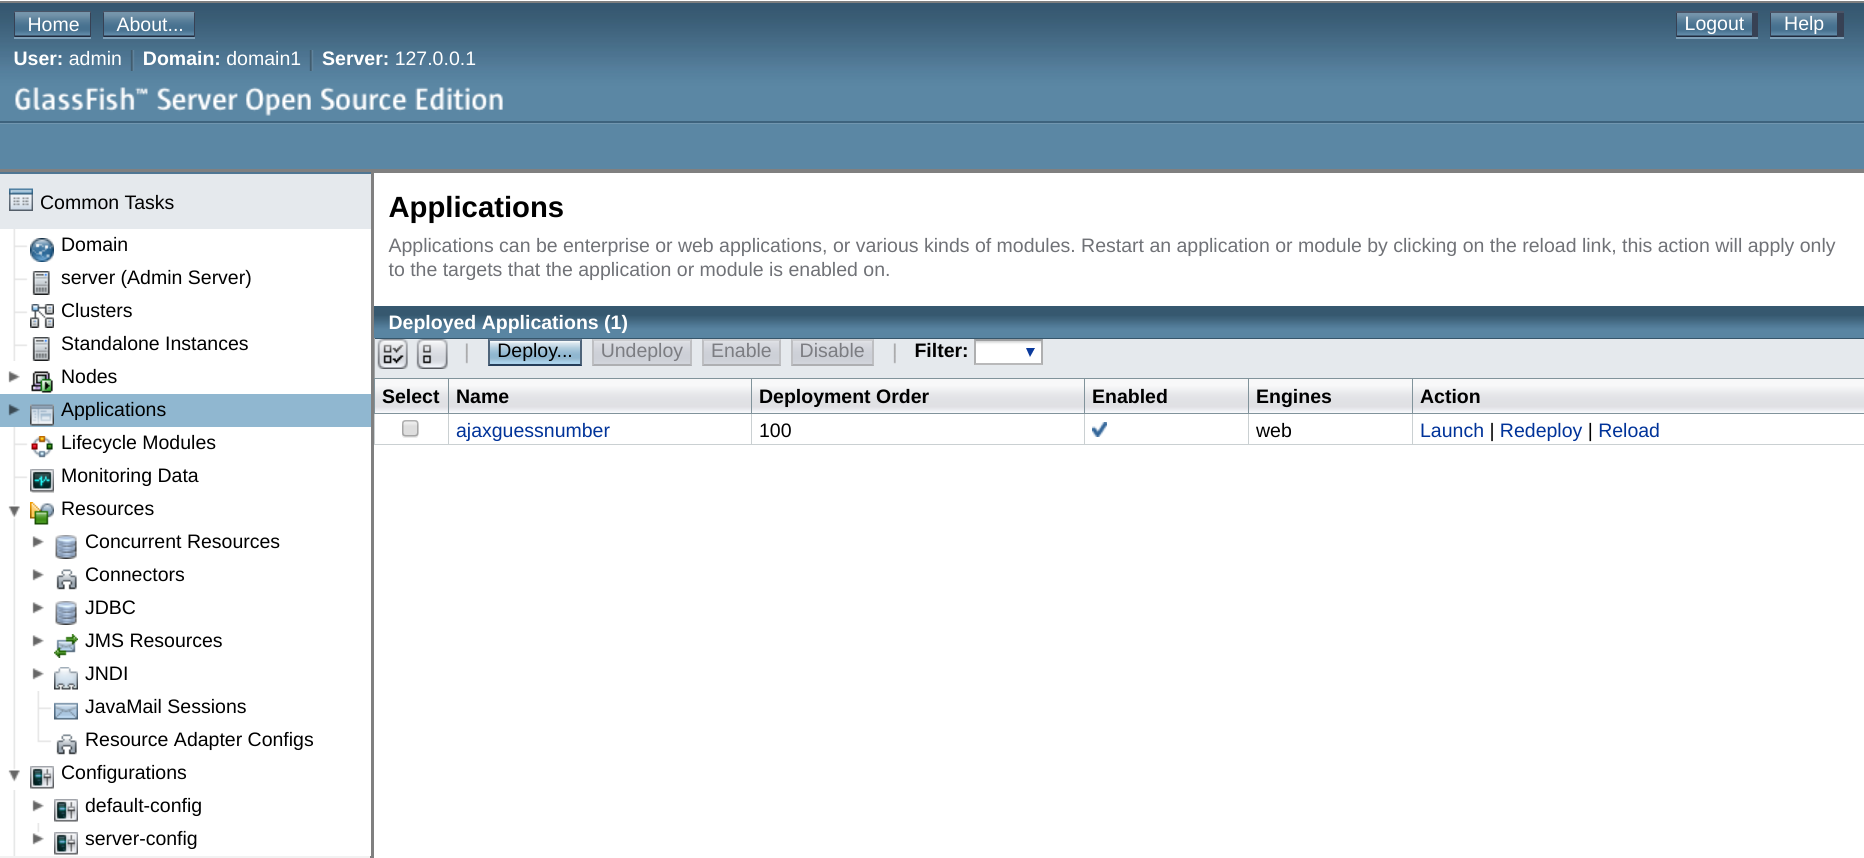
\includegraphics[width=\textwidth]{images/glassfish-apps}
    \caption{Glassfish - List all Applications}
\end{figure}

Außerdem können unter \textit{Monitoring Data} -> \textit{View Log Files} jegliche logs eingesehen werden.



\clearpage
\section{Application}

\subsection{Startseite}

Gestartet wird die Application mit dem URL Schema \texttt{localhost:8080/ajaxguessnumber[id]}:

Die Startseite der App (\texttt{getResponse} wird aufgerufen, mit \texttt{userNumber} vom Wert \texttt{null}):
\begin{figure}
    \centering
    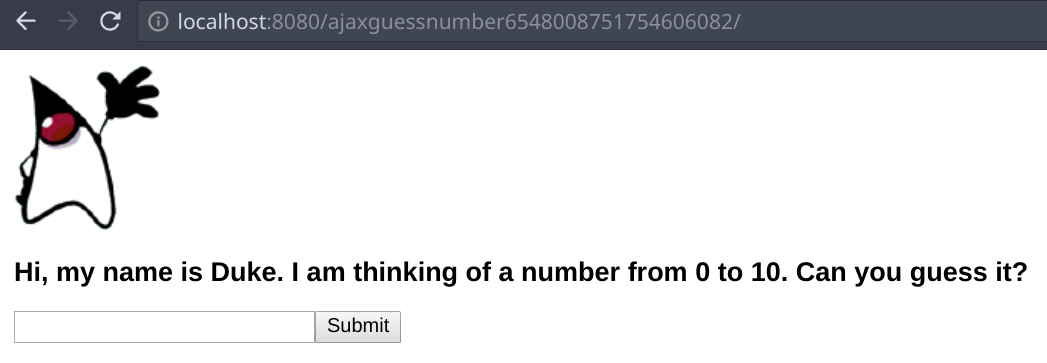
\includegraphics[width=\textwidth]{images/app-main}
    \caption{Glassfish - AjaxGuessNumber - Main Page}
\end{figure}

\subsection{Nummer raten}

Die Nummer wird überprüft, es ist jedoch die falsche (Die eigentliche Nummer ist höher):
\begin{figure}
    \centering
    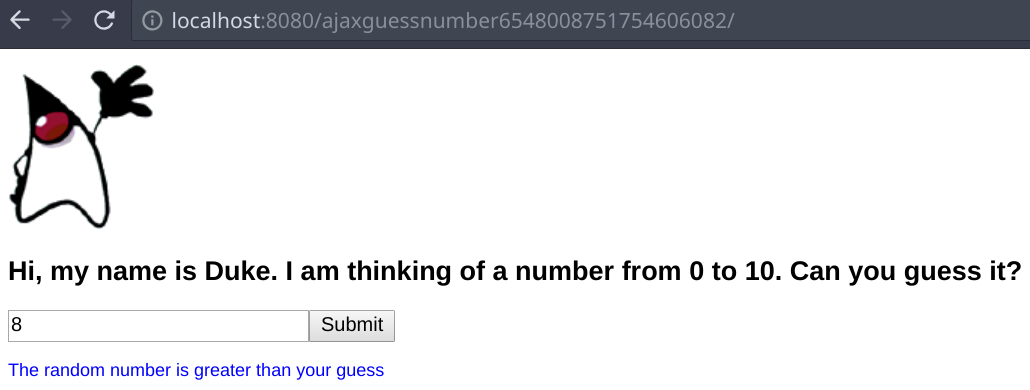
\includegraphics[width=\textwidth]{images/app-wrong-guess}
    \caption{Glassfish - AjaxGuessNumber - Wrong Number}
\end{figure}

Die Nummer wurde erfolgreich überprüft, die Benutzer Antwort ist korrekt.
\begin{figure}
    \centering
    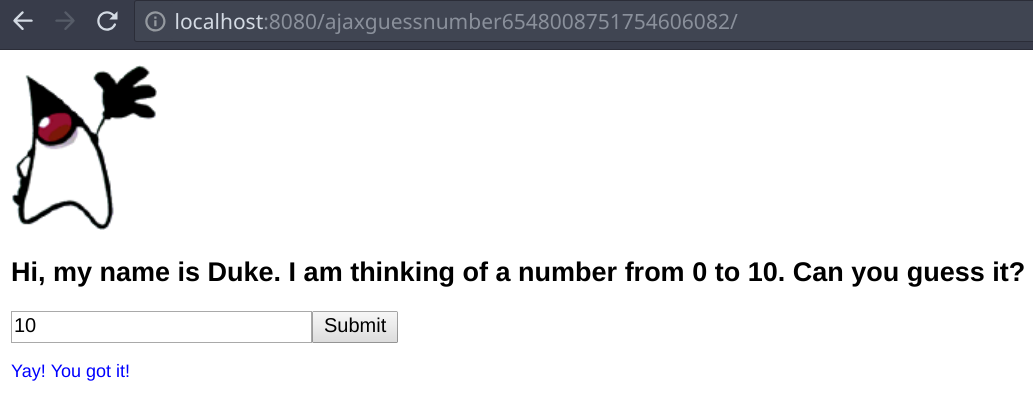
\includegraphics[width=\textwidth]{images/app-correct-guess}
    \caption{Glassfish - AjaxGuessNumber - Correct Number}
\end{figure}


\clearpage

Das Repository mit Demo Projekt, Dockerfile und Protokoll Source ist auf GitHub zu finden \cite{github:project}


\clearpage
\subsection{Persistierung}

Um die Java Persistence API (JPA) in einer JavaEE Application zu verwenden, muss die Library hinzugefügt werden (z.B.: als Maven dependency in der \texttt{pom.xml}):

\begin{code}{xml}
    <dependencies>
        <dependency>
            <groupId>org.eclipse.persistence</groupId>
            <artifactId>org.eclipse.persistence.jpa.modelgen.processor</artifactId>
            <version>${eclipselink.version}</version>
            <scope>provided</scope>
        </dependency>
    </dependencies>
\end{code}

Es muss eine \texttt{persistence.xml} Datei in dem \texttt{resources/META-INF} Ordner erstellt werden:

\begin{code}{xml}
    <?xml version="1.0" encoding="UTF-8"?>
    <persistence version="2.1" xmlns="http://xmlns.jcp.org/xml/ns/persistence" xmlns:xsi="http://www.w3.org/2001/XMLSchema-instance" xsi:schemaLocation="http://xmlns.jcp.org/xml/ns/persistence http://xmlns.jcp.org/xml/ns/persistence/persistence_2_1.xsd">
      <persistence-unit name="address-bookPU" transaction-type="JTA">
        <provider>org.eclipse.persistence.jpa.PersistenceProvider</provider>
        <jta-data-source>java:comp/DefaultDataSource</jta-data-source>
        <exclude-unlisted-classes>false</exclude-unlisted-classes>
        <properties>
          <property name="javax.persistence.schema-generation.database.action" value="drop-and-create"/>
        </properties>
      </persistence-unit>
    </persistence>
\end{code}


Eine \textbf{Entity} sieht folgendermaßen aus:

\begin{code}{java}
    @Entity
    public class Contact implements Serializable {

        private static final long serialVersionUID = -825634229676522580L;
        @Id
        @GeneratedValue(strategy = GenerationType.AUTO)
        private Long id;
        @NotNull
        protected String firstName;
        @NotNull
        protected String lastName;
        @Pattern(regexp = "[a-z0-9!#$%&'*+/=?^_`{|}~-]+(?:\\."
                + "[a-z0-9!#$%&'*+/=?^_`{|}~-]+)*@"
                + "(?:[a-z0-9](?:[a-z0-9-]*[a-z0-9])?\\.)+[a-z0-9]"
                + "(?:[a-z0-9-]*[a-z0-9])?",
                message = "{invalid.email}")
        protected String email;
        @Pattern(regexp = "^\\(?(\\d{3})\\)?[- ]?(\\d{3})[- ]?(\\d{4})$",
                message = "{invalid.phonenumber}")
        protected String mobilePhone;
        @Pattern(regexp = "^\\(?(\\d{3})\\)?[- ]?(\\d{3})[- ]?(\\d{4})$",
                message = "{invalid.phonenumber}")
        protected String homePhone;
        @Temporal(javax.persistence.TemporalType.DATE)
        @Past
        protected Date birthday;

        ...
\end{code}


Damit man auf der Datenbank (welche beliebig wählbar ist) \textbf{CRUD} (Create Update Read Delete) Operationen ausführen kann, wählt man zwischen dem EntityManager, einer Repository oder einer \textbf{Facade}.

Hierbei wird eine abstrakte generische Facade definiert:

\begin{code}{java}
    public abstract class AbstractFacade<T> {
        private Class<T> entityClass;

        public AbstractFacade(Class<T> entityClass) {
            this.entityClass = entityClass;
        }

        protected abstract EntityManager getEntityManager();

        // CREATE
        public void create(T entity) {
            getEntityManager().persist(entity);
        }

        // UPDATE
        public void edit(T entity) {
            getEntityManager().merge(entity);
        }

        // DELETE
        public void remove(T entity) {
            getEntityManager().remove(getEntityManager().merge(entity));
        }

        // READ
        public T find(Object id) {
            return getEntityManager().find(entityClass, id);
        }

        ...
\end{code}

Um eine Facade für die \textit{Entity} \texttt{Contact} zu erstellen, wird die \texttt{ContactFacade} folgendermaßen implementiert:

\begin{code}{java}
    @Stateless
    public class ContactFacade extends AbstractFacade<Contact> {
        @PersistenceContext(unitName = "address-bookPU")
        private EntityManager em;

        @Override
        protected EntityManager getEntityManager() {
            return em;
        }

        public ContactFacade() {
            super(Contact.class);
        }
    }
\end{code}

In \textbf{EJB} bedeutet \texttt{@Stateless}, dass es keine wirkliche Instanzen gibt sondern alles einen neuen Context (oder \texttt{EntityManager}) erstellt.

Die API wird den \texttt{EntityManager} automatisch erstellen, da er die Annotation \texttt{@PersistenceContext} besitzt.
